\chapter{Secure Bootstrapping}
\label{ch:secureBootstrapping}
The term ``Bootstrapping" is used in a spectrum of contexts including Computing, Law, Finance\footfullcite{bs-wiki}. It is inspired from the late idiom ``to pull oneself up by one's bootstraps" which means to succeed or elevate yourself without any outside help. In the context of Networking, bootstrapping is an initial procedure between an unconfigured devices which intend to communicate with a network for the first time. Its goal is to provide the device with the required information that enables it to establish subsequent secure communication channels with the desired network. Such information can be certificates, configurations, and metadata.
\par
Integrity and confidentiality of information flow between the two ends of the communication are are what defines end to end secure channels. Authentication, whether unilateral or mutual, is another fundamental aspect to achieve channel security. Existing protocols, such as \gls{tls}, can achieve End-to-end security between parties. However, analogous protocols rely digital certificates and credentials which are managed by local or third party \gls{pki}. Therefore to ensure correct and secure execution of protocols certificates must be securely provisioned to their corresponding identities. Typically at the manufacturing phase, the manufacturer usually installs globally unique manufacturer provided identifiers known as the \gls{idevid} \cite{5367679}. Its main use is for identity verification purposes and it should not be used to enforce data integrity nor confidentiality. Upon successful completion of the bootstrapping process, the device should posses identifiers that allows for subsequent establishment of secure channels with the network domain. An identifier in this set of identifiers is known as \gls{ldevid} \cite{5367679}.
\par
Bootstrapping approaches differ in the degree of manual user involvement and the amount of information on the device which must be pre-configured by the manufacturer. The survey by Sethi et al. \cite{irtf-t2trg-secure-bootstrapping-00} provides a classification for Bootstrapping mechanisms into general categories: Managed methods, \gls{p2p} and Ad-hoc methods, Opportunistic methods, and Hybrid methods.
\begin{itemize}
	\item \textit{Managed methods}: These bootstrapping approaches count on pre-established credentials and trust anchors for authentication and security. The required initial information and cryptographic material can be acquired either at manufacture time in the factory, or through \gls{oob} means, e.g. using a smart card or a USB. Examples of this method are \gls{eap-tls} \cite{eap-tls} and \gls{gba} \cite{gba}.
	
	\item \textit{\gls{p2p} methods}: Contrary to managed methods, these bootstrapping methods do not rely on any pre-established cryptographic material or information. Instead, the bootstrapping protocol results in credentials being established for subsequent secure communication. Typically, resulting credentials are authenticated using an \gls{oob} channel. This category of methods may be utilized if the manufacturer is incapable or untrustworthy to generate the desired credential.
	
	\item \textit{Opportunistic methods}: Unlike previous methods where the authenticity of the initially presented identity is verified, approaches which fall under this category rely on verification of the continuity of the initial identity provided. Bergmann et al. \cite{simplekeys} have developed a secure bootstrapping mechanism that is an example of this category. 
	
	\item \textit{Hybrid methods}: A wide range of deployed approaches use components from both managed and \gls{p2p} methods. Such approaches are categorized as hybrid methods.	
\end{itemize} 

This chapter discusses two voucher-based bootstrapping protocols that aim at being zero touch protocols by eliminating the user interference. These protocols are \gls{brski} \cite{brski} and \gls{sztp} \cite{sztp}. Both protocols fall under the managed methods category.

%brski section
\section{\acrfull*{brski}}
%intro
\gls{brski} is a product of the ANIMA working group of the \gls{ietf}. It is an automated bootstrapping protocol that enables an unconfigured device to discover and securely join an unfamiliar network domain it is installed in. \gls{brski} results in the device acquiring an X.509 root certificate to authenticate the network domains' elements and establish consecutive secure channels. Moreover, the device can use the obtained certificate to perform further certificate enrollment protocols, like \gls{est} \cite{rfc7030}. \gls{brski} is capable of realizing a large scale of thousands of devices in a risk prone environment. For example, customer devices provided by ISPs which are directly shipped to the customers.

\subsection{Architecture Overview}

The environment of \gls{brski} is composed of three general entities: the network domain, the pledge, and the manufacturer services. Figure \ref{brski-architecture} shows an overview of the protocols architecture.

\begin{figure}[H]
	\centering
	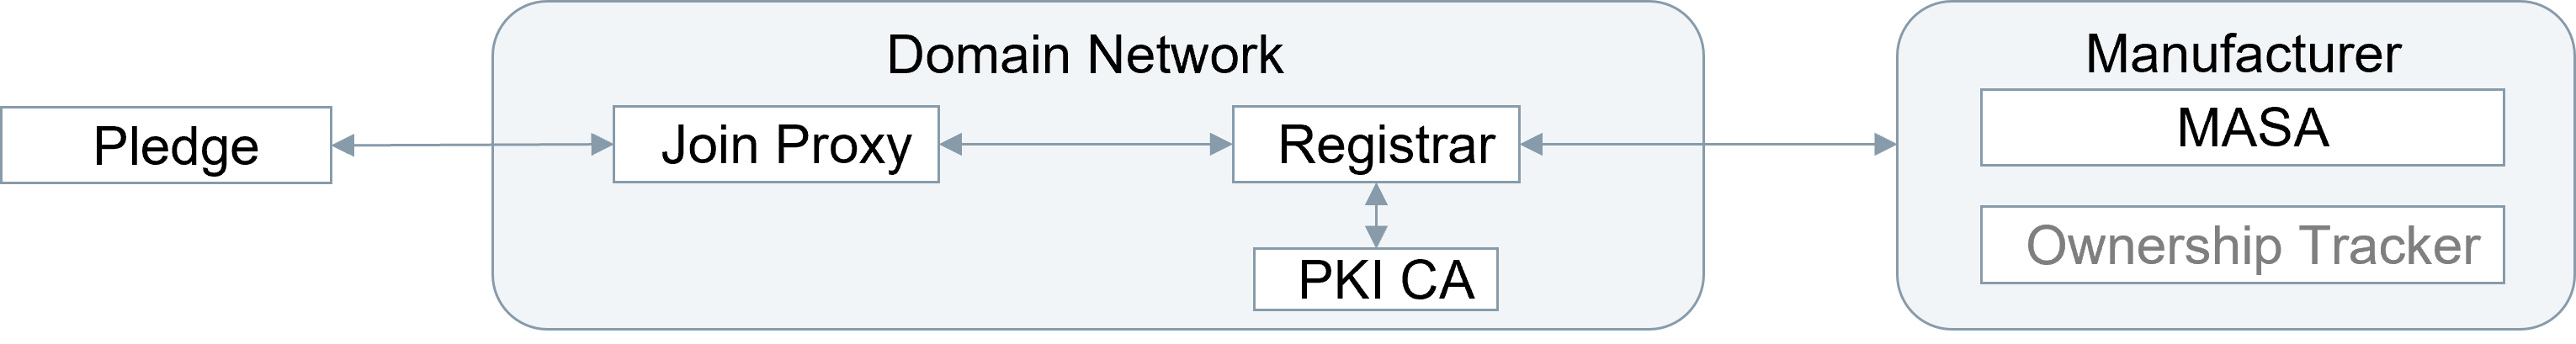
\includegraphics[scale=0.4]{Images/brski-overview.png}
	\caption{BRSKI Architecture.}
	\label{brski-architecture}
\end{figure}

The network domain is the domain of the alleged new owner of the device, i.e the network that is expecting the device to be connected to it. The domain is a network of entities who share a common local trust anchor. 
It incorporates a \gls{pki} to govern the issuance of digital certificates to provide unique digital identifiers for clients and establish end-to-end security. 
\par
A join proxy is another component of the domain. It helps with the discovery of pledges that intend to join the network. In addition, it is responsible for discovering the domain registrar(s) and determining the proxy mechanisms supported by the registrar and utilizing the lowest impact mechanism.
Pledge discovery methods can be classified into passive and active methods. 
GRASP flooding \cite{rfc8990} is a pledge passive discovery method for autonomic networks \cite{kephart2003vision}. It is short for GeneRic Autonomic Signaling Protocol. It is used for signaling between autonomic service agents. GRASP provides discovery, flooding, synchronization, and negotiation functionalities for the technical objectives through respective GRASP messages. Pledge discovery via GRASP multicast flooding is the normative and mandatory method for \gls{brski}.
On the other hand, DNS-based Service Discovery \cite{rfc6763} over Multicast DNS \cite{rfc6762} as well as DHCP \cite{rfc2131} are pledge active discovery methods. They can be used as secondary discovery methods in parallel to GRASP.
Moreover, A proxy provides HTTPS connectivity and forwards messages without examination between a pledge and a registrar in the network, and without interfering with the protocol messages.
\par
A pledge is an unconfigured device attempting to join the network domain. Its goal is to be securely bootstrapped in a zero-touch fashion. To achieve this goal, the pledge establishes a TLS connection with one or more of the domain's registrars through the domain's proxy. It is necessary for the pledge and the registrar to establish mutual authentication. A manufacturer installed \gls{idevid} is used for pledge authentication to the domain's registrar. It is installed during the manufacturing process and includes certificates signed by the manufacturer and unique identifiers that represent the pledge, in addition to, the pledge unique serial number given by the manufacturer. It is recommended that The provided certificates are used for authentication with the registrar and the signing of voucher requests. The unique serial number is used in vouchers and voucher requests to ensure linkability. 
\par
A registrar is an element of the domain that is responsible to carry out the bootstrap process for the pledge. Also, it can be considered as the \gls{ra} for the domain's \gls{pki}. A domain can have one or more registrars which all have to be recognized by the domain proxy. If the pledge is capable to concurrently connect to multiple registrars, it is advisable to do so as this protects against a malicious proxy attempting a \gls{dos} attack like Slowloris.
\par
A manufacturer is the entity that produced the device and set up its initial configuration (IDevID). It provides two distinct services: the \gls{masa} service and ownership tracking and validation.
MASA can be a third party service that signs the vouchers issued for the bootstrapping process. It is also responsible for providing a repository for audit-log information of bootstrapping events. The service is contacted each time a pledge performs a zero-touch bootstrap in an attempt to enroll into a domain. It takes the decision whether or not issue the voucher according to the MASA policy. Voucher issuance could be done blindly at the lowest security level or it could be tightly bound to the sales channel that verifies the actual ownership of the domain. Hence, the manufacturer can provide protection against stolen devices or illegitimate resale of devices by declining voucher issuance to the suspected pledge.
\par
Ownership tracking and validation is an optional manufacturer service. It is supposed to log all claim attempts and to know which device is owned by which domain and provide such information to registrars. A verified log entry indicates that the pledge was issued a voucher as a result of positive verification of ownership.

\subsection{Protocol Details}
This section describes the message sequence of BRSKI illustrated in figure \ref{brski-protocol} and elaborates on content of the exchanged messages. The numbering sequence referenced through this section refers to the message numbers in figure \ref{brski-protocol}.

\begin{figure}[htbp]
	\centering
	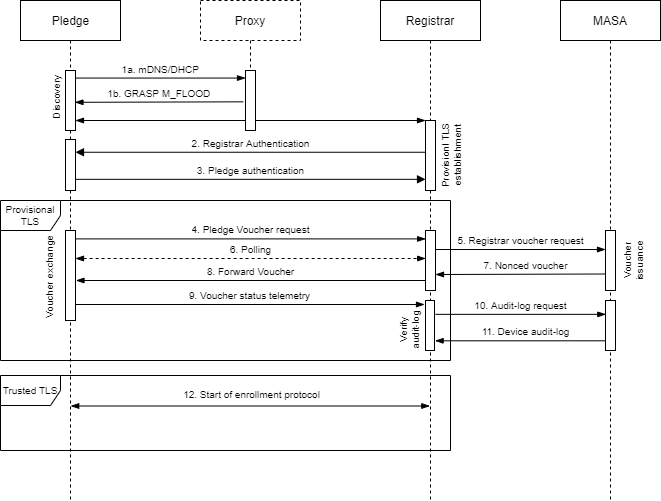
\includegraphics[scale=0.4]{Images/brski-architecture.png}
	\caption{A successful BRSKI protocol run.}
	\label{brski-protocol}
\end{figure}

\begin{itemize}
	\item \textit{Message 1a, 1b (Discovery phase):} It is the first phase of the protocol where the pledge identifies the domain proxy. This can be performed by a pledge initiated mechanism as in message (1a) or via a proxy initiated mechanism as in message (1b). After successful discovery, the pledge can address a domain registrar through the proxy. A proxy does not assume any specific TLS version.

	\item \textit{Message 2, 3 (Provisional TLS establishment):} The pledge attempts to establish a TLS channel with each discovered registrar to ensure End-to-End security. The pledge must not use any TLS version lower than TLS 1.2, while TLS 1.3 is the encouraged version to be used. To establish the channel, mutual authentication has to be performed.
	At first, in message (2), the pledge receives the registrar's server certificate. However, the pledge does not posses any trust anchors to verify it yet. Therefore, the pledge accepts the registrar's certificate provisionally.
	Next in message (3), the pledge is authenticated via the installed IDevID. The registrar must be able to verify the provided certificate, however the distribution of the trust anchors for this task is out-of-scope of BRSKI.
	Meaning, the information received by the pledge must be untrusted, although it is in a TLS channel, till a trusted trust anchor to verify the certificate is received. 

	\item \textit{Message 4:} Having established a secure provisional TLS channel, the pledge initiates the voucher exchange by sending a pledge voucher request to the registrar in message (4). The request must contain a unique nonce per bootstrapping attempt to protect against replay attacks. Also, the request contains the `proximity-registrar-cert' and the pledge serial number.
	The `proximity-registrar-cert' is the \gls{ee} certificate of the registrar which is also used to establish the provisional TLS channel. Pledge serial number is a manufacturer defined unique identifier for each device. It is different from the IDevID certificate serial number. Since not all devices have a real-time clock, depending on the device capabilities, the request is recommended to have the 'created-on' value. Finally, the request must be signed using the pledge's IDevID certificate.
	\par
	The registrar authorizes the pledge based on the authenticated information presented in the pledge's IDevID and the registrar's policy. The policy can be either to allow any device from a specific vendor, to allow any device of a specific type, or to allow a specific type of devices from a specific vendor.
	
	\item \textit{BRSKI-MASA TLS channel:} The registrar initiates a TLS 1.2 or newer channel with the MASA where all subsequent communication between the two parties occur within this secure channel. The MASA URL is obtained from the pledge IDevID, as mentioned earlier. To authenticate the MASA, the registrar should be configurable with trust anchors on a per vendor MASA basis as part of the sales process. Moreover, the registrar should also support client authentication mechanisms such as TLS client certificate, HTTP Basic, Digest, or \gls{scram}; however TLS Client Certificate based authentication is the recommended method.
	
	\item \textit{Message 5:} After obtaining the pledge's voucher request, the registrar constructs a registrar voucher request that is sent to the MASA to obtain a voucher for the pledge. The registrar voucher request is a JSON document that is signed using a CMS structure. The JSON document encapsulates the pledge voucher request CMS object that was sent to the registrar and is referred to as `prior-signed-voucher-request'. Moreover, the request contains the `created-on' field which holds the timestamp the request was formed on. In addition, it consists of other fields which relate to the pledge request like the pledge serial number, the nonce used produced by the pledge and used in the pledge request, and `idevid-issuer' field which holds the issuer value of the pledge IDevID certificate. The registrar includes some certificates in the registrar voucher request CMS object as well. Those certificates are used by the MASA to be pinned into the voucher to be later used by the pledge as a trust anchor for authenticating the domain registrar. Therefore, the certificates enclosed by the registrar in the request have to be part of the chain it wishes the MASA to pin in the voucher. Hence the specificity of the attached certificates is considerably significant. A `pinned-domain-cert' can be as specific as the registrar's TLS \gls{ee} certificate. On the other hand, if it is as general as a public webPKI \gls{ca} it could permit any entity that possess a certificate issued by that authority to claim ownership of the device.
	\par
	On the other hand, the pledge might not be available at the time of deployment to send a pledge voucher request, or the registrar speculates to not being able to reach the MASA at the time of deployment where the pledge will be available. Such use cases justify the need for nonceless registrar voucher request. In these cases, the previous message (4) would not exist. To formulate this request, the registrar has to acquire the pledge's serial number and IDevID issuer, however, they are obtained through out-of-band means. Subsequently, the nonce field of the request is omitted.
	
	\item \textit{Phase 6 (Polling)}: Before processing the pledge's request, the registrar may send the pledge an HTTP 202 response message which indicates that the request received earlier has been accepted for processing however processing is not yet complete. This response initiates a polling phase between the pledge and the registrar. A ``Retry-After" field is specified within the headers of the registrar's response that indicates the minimum time for the pledge to wait before asking for a response for the voucher request sent earlier. After the specified waiting time, the pledge polls the response by resending the exact same request and must not change the nonce nor sign a new voucher request. If the pledge is simultaneously trying to bootstrap itself with several registrars of the network, it can be overwhelming for the pledge to keep track of all the ``Retry-After" times. Therefore, a pledge may ignore the specified interval and follow a hard-coded ``Retry-After" interval. A pledge should be able to hold the retry state for a maximum of 4 days.
	
	\item \textit{Message 7:} upon receiving the voucher request, the MASA performs a set of checks to decide weather to issue the requested voucher. Given the fact that vouchers have a short lifetime, the request may be from a registrar that has been issued a voucher previously, i.e a voucher renewal request. In this case, the request should be automatically authorized by the MASA.
	\par
	 The MASA extracts the certificate chain attached in the signed CMS object. If the domain CA is unknown to the MASA it is considered as a temporary trust anchor as the intention is not to authenticate the message rather to establish consistency of the domain PKI. According to the MASA's policy, it decides which certificate of the chain supplied by the registrar it chooses to pin. It may be the farthest certificate of the chain, or it may be as close as the \gls{ee} TLS certificate of the registrar. If revocation information is available for that certificate, it must be checked by the MASA to prevent issuance of new or renewed vouchers to unauthorized registrars. Next, the CMS signature is validated using the domain's CA extracted from the voucher request. Also, the signing certificate is verified to contain the `id-kp-cmcRA' Extended Key Usage. This ensures that the signer is an entity that is authorized to be a registrar of the domain. Hence, assures domains that a MASA only accepts requests from domain registrars. 
	 \par
	 In case of nonceless requests, It is mandatory for the MASA to authenticate the registrar. The decision to issue a noncless voucher is taken according to the MASA policy that is out of scope.
	 \par 
	 In case of nonced voucher requests, the MASA verifies that the `prior-signed-voucher-request', enclosed in the registrar request, contains a `proximity-registrar-cert' that is coherent to the certificate used to sign the registrar voucher request. Moreover, the nonce is verified to be consistent between the registrar voucher request and the `prior-signed-voucher-request'.
	 \par
	 Subsequent to a successful validation of the request, the MASA responds with an issued voucher in message (6). Any issued voucher by the MASA is recorded in the audit-log. Otherwise if a problem occurs, a response with the appropriate http signaling as described in \cite{brski}. For example, a 403 status code response if the voucher request is not signed correctly, or a 406 status code response if the requested voucher type or algorithms cannot be issued due to the MASA's awareness that such pledge is not capable of processing them.
	 
	\item \textit{Message 8:} The registrar evaluates the received voucher solely for transparency and future audit-log verification. The received voucher is forwarded to the pledge without any interference or modification from the registrar.

	\item \textit{Message 9:}
 	 After the pledge successfully receives a voucher, the pledge must indicate its status regarding the voucher to the domain. This occurs by sending a status message to the registrar. The pledge decides weather to accept the voucher or not through the voucher validation process. If acceptable, the message should contain the version of BRSKI and a boolean status field to indicate the acceptance status. In case of an unacceptable voucher or a failure, the pledge is expected to fail gracefully. The message should contain a Reason field with a string commenting on the cause. Nevertheless, the Reason should not be excessively descriptive as it may be sent to an unauthenticated and potentially malicious registrar.
	 \par
	 Bearing the voucher, the pledge verifies its validity. It verifies the signature using the manufacturer installed MASA trust anchor. It verifies also that the serial number enclosed in the voucher matches its own. For nonced vouchers, the pledge verifies the voucher nonce corresponds to the nonce it sent earlier in the voucher request. However nonceless vouchers can be accepted according to pledge local policy. The pledge can be configured to always accept nonceless vouchers to realize the use case where the MASA is unreachable at the time of pledge deployment.
	 \par
 	 A pledge could be operating in other similar security reduced mode that skip voucher validation in favor of offline or emergency touch-based deployment bootstrapping procedures. For example, \gls{tofu} or physical presence methods such as the use of serial console or depressing a physical button during bootstrapping. However, \gls{tofu} must not be available unless a hardware-assisted \gls{nea} is supported. Meanwhile, it is only recommended for other methods of skipping voucher validation. This recommendation serves as a prevention against unintended use of offline methods when autonomic methods fail or are unavailable.
	 \par
	 Upon successful verification of the voucher, the voucher's pinned-domain-cert should be considered by the pledge as a trust anchor. The current provisional TLS connection between the pledge and the registrar is evaluated using the obtained trust anchor. The pledge verifies the registrar's TLS server certificate using the trust anchor's public key. If the registrar's credentials could be verified, either by directly matching the server certificate or through verifying a higher certificate in its chain, the pledge trust the TLS connection and it is not considered provisional any further.
	 
	\item \textit{Message 10:} After receiving the pledge status telemetry message, the registrar requests the MASA audit-log from the MASA. The log data helps the registrar make a knowledgeable decision regarding further proceeding of the bootstrapping process. The decision making criteria is based upon the security requirements of the registrar domain. Hence, the criteria is out of the protocol's scope.
	The request content is the exact same registrar voucher-request sent earlier to the MASA, but is directed through a different URI specific for requesting the audit log, which is ``/.well-known/brski/requestauditlog". Reusing the same message minimizes the required cryptographic and message operations on both ends. The registrar may reuse the cached voucher request and the MASA may take advantage of its internal state to correlate the message with the already verified request averting additional operations.
	
	\item \textit{Message 11:} 
	A MASA can infer the proper pledge log to be prepared from the ``idevid-issuer" and the ``serial-number" information included in the received request of the previous message. Instead of immediately responding with the audit-log, the MASA can a HTTP 201 ``Created" response with a URL in the ``Location" header field redirecting to actual audit-log. The response log is a JSON format document consisting of all the log entries associated with the pledge. Nevertheless, a MASA that sends out URLS has to ensure they are unpredictable to avoid enumeration attacks against device audit-logs.
	\par
	The log format structure consists of several entries: ``version", ``events", and ``truncation". ``version" is an integer value representing the log format version. ``events" is an array of event objects that are associated to the device. 
	Each of the event objects is comprised of a set of entries. The ``date" entry represents the event's timestamp in the format according to \cite{rfc3339}. 
	The ``domainID" is a unique identifier for the domain's registrar that encodes the pinned-domain-cert's SubjectKeyIdentifier or SPKI fingerprint in base64. A ``nonce", if exists, is a base64 encoding of the same nonce used in the voucher request and issued voucher. If it is a nonceless voucher, then the field should preferably be set to null rather than omitting it. 
	The ``assertion" field indicates the level of verification with which the MASA issued the voucher. It can have one of three values: ``verified", ``logged", and ``proximity"; the latter being the one supported by this protocol.
	``truncated" field shows the number of event truncations for the specified domainID.
	Lastly, since audit-logs can be arbitrarily large, duplicated or old entries may be truncated as an optimization for the log structure. The ``truncation" entry contains meta-information about truncated entries such as ``nonced duplicates", ``nonced duplicates", and ``arbitrary".
	\par
	On the registrar side, the received audit-log is vetted for discrepancies and unexpected behavior like the pledge previously imprinting to an unexpected domain or whether a certain domain possesses a nonceless voucher and can reset the device anytime. If the registrar's audit-log verification is successful, then the bootstrapping process is complete.
	
	\item \textit{Message 12:} 
	At this point, the pledge has a trust anchor allowing it to verify the registrar, as well as a trusted TLS channel between them. Therefore the environment is suitable to start a certificate enrollment protocol after which the pledge obtains digital certificates that authenticate it to the domain and authorize it to utilize the relevant domain services.
	\par
	BRSKI is described as an extension for \gls{est} that provides automated proposal instead of the originally manual authentication method that relies on the intervention of a human user. Hence it is recommended for a pledge to use EST following BRSKI as a certificate enrollment protocol as it is considered a harmonious integration.
	\par 
	Nonetheless, the succeeding certificate enrollment protocol is not limited to \gls{est}, however, a variety of certificate enrollment protocols can be used. Using \gls{est} is an example of a pull model where the EST server is the protocol initiating party. As an example of the push model architecture, \gls{cmp} can be used as the certificate enrollment protocol since the \gls{ee} is the initiating party of the protocol. 
	

\end{itemize}











%sztp section
\section{\acrfull*{sztp}}

\section{Protocols Comparison}
